
% -- --------------------------------------------------------------------------------------------------- -- %
% -- posteR-knitR: Templates for LaTeX (Beamer) and R Programming (knitR) for research posters           -- %
% -- --------------------------------------------------------------------------------------------------- -- %
% -- Description: Beamer poster LaTeX format and knitR R package bindings for research posters           -- %
% -- poster.rnw: File with LaTeX and R codes                                                             -- %
% -- Author: IFFranciscoME - if.francisco.me@gmail.com                                                   -- %
% -- license: MIT License                                                                                -- %
% -- Repository: https://github.com/IFFranciscoME/posteR-knitR                                           -- %
% -- --------------------------------------------------------------------------------------------------- -- %

\documentclass{postertheme}\usepackage[]{graphicx}\usepackage[]{color}
% maxwidth is the original width if it is less than linewidth
% otherwise use linewidth (to make sure the graphics do not exceed the margin)
\makeatletter
\def\maxwidth{ %
  \ifdim\Gin@nat@width>\linewidth
    \linewidth
  \else
    \Gin@nat@width
  \fi
}
\makeatother

\definecolor{fgcolor}{rgb}{0.345, 0.345, 0.345}
\newcommand{\hlnum}[1]{\textcolor[rgb]{0.686,0.059,0.569}{#1}}%
\newcommand{\hlstr}[1]{\textcolor[rgb]{0.192,0.494,0.8}{#1}}%
\newcommand{\hlcom}[1]{\textcolor[rgb]{0.678,0.584,0.686}{\textit{#1}}}%
\newcommand{\hlopt}[1]{\textcolor[rgb]{0,0,0}{#1}}%
\newcommand{\hlstd}[1]{\textcolor[rgb]{0.345,0.345,0.345}{#1}}%
\newcommand{\hlkwa}[1]{\textcolor[rgb]{0.161,0.373,0.58}{\textbf{#1}}}%
\newcommand{\hlkwb}[1]{\textcolor[rgb]{0.69,0.353,0.396}{#1}}%
\newcommand{\hlkwc}[1]{\textcolor[rgb]{0.333,0.667,0.333}{#1}}%
\newcommand{\hlkwd}[1]{\textcolor[rgb]{0.737,0.353,0.396}{\textbf{#1}}}%
\let\hlipl\hlkwb

\usepackage{framed}
\makeatletter
\newenvironment{kframe}{%
 \def\at@end@of@kframe{}%
 \ifinner\ifhmode%
  \def\at@end@of@kframe{\end{minipage}}%
  \begin{minipage}{\columnwidth}%
 \fi\fi%
 \def\FrameCommand##1{\hskip\@totalleftmargin \hskip-\fboxsep
 \colorbox{shadecolor}{##1}\hskip-\fboxsep
     % There is no \\@totalrightmargin, so:
     \hskip-\linewidth \hskip-\@totalleftmargin \hskip\columnwidth}%
 \MakeFramed {\advance\hsize-\width
   \@totalleftmargin\z@ \linewidth\hsize
   \@setminipage}}%
 {\par\unskip\endMakeFramed%
 \at@end@of@kframe}
\makeatother

\definecolor{shadecolor}{rgb}{.97, .97, .97}
\definecolor{messagecolor}{rgb}{0, 0, 0}
\definecolor{warningcolor}{rgb}{1, 0, 1}
\definecolor{errorcolor}{rgb}{1, 0, 0}
\newenvironment{knitrout}{}{} % an empty environment to be redefined in TeX

\usepackage{alltt}

\usepackage{lipsum}                                % Package for dummy text
\usepackage[absolute, overlay]{textpos}            % Figure placement
\usepackage{graphicx}
\usepackage{float}

\setlength{\TPHorizModule}{\paperwidth}
\setlength{\TPVertModule}{\paperheight}

\title{T-Fold Sequential Validation Technique for Out-Of-Distribution Generalization with Financial
       Time Series Data}

\vskip4cm

\author {Juan Francisco Muñoz-Elguezabal \inst{1} \and Juan Diego Sánchez-Torres \inst{1}}
\institute {\inst{1} Western Institute of Technology and Higher Education (ITESO)}

% -- ------------------------------------------------------------------------- CODE 1: SOME CALCULATIONS -- %
% -- ------------------------------------------------------------------------- ------------------------- -- %



\IfFileExists{upquote.sty}{\usepackage{upquote}}{}
\begin{document}

\begin{frame}

% -- -------------------------------------------------------------------------------------- ----------- -- %
% -- -------------------------------------------------------------------------------------- ----------- -- %

\begin{columns}[onlytextwidth]
  
  \begin{column}{1 \textwidth - 0.01 \textwidth}
    \begin{block}{Presented Case Specifications}

    \textbf{Hipothesis:}
      There exists a set of conditions under which a cross-validation process can be defined and conducted in
      order to achieve Out-Of-Sample and Out-Of-Distribution Generalization when performing a Predictive
      Modeling Process using Financial Time Series Data.
      
    \textbf{Dataset:}
      Continuous futures prices of the UsdMxn (U.S. Dollar Vs Mexican Peso),
      extracted from CME group MP Future Contract. Prices are Open, High, Low, Close
      in intervals of 8 Hours, \textbf{OHLC} data. GMT timezone-based and a total of 66,500 
      from 2010-01-03 18:00:00 to 2021-06-14 16:00:00.
    
    \textbf{Experiment:}
      A classification problem is formulated as to predict the target variable, $CO_{t+1}$, which is defined
      as the $\text{sign}(Close_{t+1} - Open_{t+1})$. For the explanatory variables, the base definition is to
      use only those of endogenous nature, that is, to create them using only \textbf{OHLC} values.
  
    \end{block}
  \end{column}
\end{columns}

% -- -------------------------------------------------------------------------------------- ----------- -- %
% -- -------------------------------------------------------------------------------------- ----------- -- %

\begin{columns}[onlytextwidth]
  
  \begin{column}{.33 \textwidth - 0.01 \textwidth}
    \begin{block}{A discrete multi-period characterization}
    
      Let $V_{t}$ be the value of a financial asset at any given time $t$, and $S_{t}$ as a discrete 
      representation of $V_{t}$ if there is an observable transaction $Ts_{t}$. Similarly, if there is 
      a set of discrete $Ts_{t}$ observed during an interval of time $T$ of $n = 1, 2, ... , n$ units of time, 
      $\left\{ S_{T} \right\}_{T=1}^{n}$, can be represented by
      $OHLC_{T}: \left\{ Open_{t}, High_{t}, Low_{t}, Close_{t} \right\}$. The frequency of sampling $T$,
      can be arbitrarly defined. 
      
    \end{block}
  \end{column}
  
  \begin{column}{.33 \textwidth - 0.01 \textwidth}
  \begin{block}{OHLC representation}
  
      For every $OHLC_{T}: \left\{ Open_{t}, High_{t}, Low_{t}, Close_{t} \right\}$:
      
      \textbf{Timestamp}: The date and time for each interval. \\
      \textbf{Open}: The first price of the interval. \\
      \textbf{High}: The highest price registered during the interval. \\
      \textbf{Low}: The lowest price registered during the interval. \\
      \textbf{Close}: The last price of the interval.

  \end{block}
  \end{column}

  \begin{column}{.33 \textwidth - 0.01 \textwidth}
    \begin{block}{Candlestick Visual Representation \footnotesize \textit{(Figure 1)}}
    \vskip-.4in
          \begin{figure}
            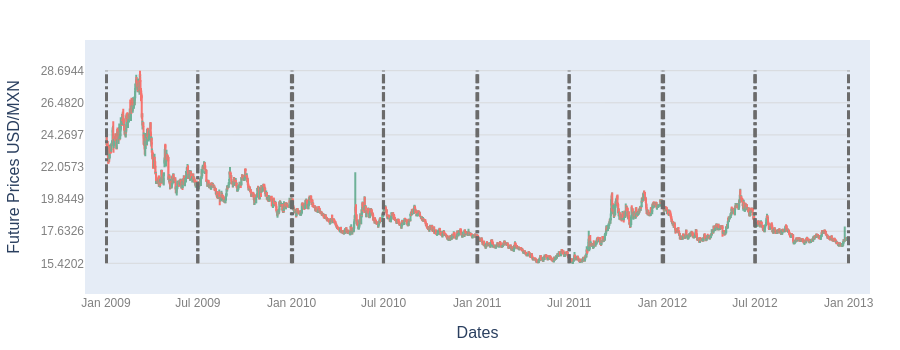
\includegraphics[width=34cm, height=10cm,keepaspectratio=true]{figures/plot-ohlcprices.png}
          \end{figure}
    \end{block}
  \end{column}

\end{columns}

% -- -------------------------------------------------------------------------------------- ----------- -- %
% -- -------------------------------------------------------------------------------------- ----------- -- %

\begin{columns}[onlytextwidth]
  
  \begin{column}{.25 \textwidth - 0.01 \textwidth}
    \begin{block}{Linear Variables}
      
      \textbf{micro-volatility:}  $ \rightarrow HL_{t}$ \\
      \textbf{micro-trend:} $ \rightarrow CO_{t}$ \\
      \textbf{micro-uptrend:} $ \rightarrow HO_{t}$ \\ 
      \textbf{micro-downtrend:} $ \rightarrow OL_{t}$
      
    \end{block}
  \end{column}

  \begin{column}{.5 \textwidth - 0.01 \textwidth}
    \begin{block}{Autoregressive Variables}
        
      Fundamental operations: $MA_t$, lag: $LAG_t$, standard deviation: $SD_t$ and cumulative
      sumation: $CSUM_t$. This operations where applied to the past linear features: 
      $\left\{ OL \right\}_{t-k}$, $\left\{ HO \right\}_{t-k}$, $\left\{ HL \right\}_{t-k}$,
      $\left\{ HLV \right\}_{t-k}$, $\left\{ COV \right\}_{t-k}$, $\left\{ VOL \right\}_{t-k}$
      for values of $k = 1, 2, ... K$, with $K$ as a proposed \textit{memory} parameter.

    \end{block}
  \end{column}
  
  \begin{column}{.25 \textwidth - 0.01 \textwidth}
    \begin{block}{Target variable}
    
      A continuous variable prediction (regression problem), into
      a discrete variable prediction (classification problem):
      
      $\hat{y}_{t} = sign \left\{ CO_{t} \right\}$

    \end{block}
  \end{column}
  
\end{columns}

% -- -------------------------------------------------------------------------------------- ----------- -- %
% -- -------------------------------------------------------------------------------------- ----------- -- %

\begin{columns}[onlytextwidth]
  
  \begin{column}{.25 \textwidth - 0.01 \textwidth}
    \begin{block}{T-Fold-SV \footnotesize \textit{(Steps)}}
        
      \footnotesize
      
      \textbf{1.- Fold Formation} \\
        Depends on labeling, can be calendar based.\\
      \textbf{2.- Target and Feature Engineering} \\
        In-Fold exclusive or Global and then divide.\\
      \textbf{3.- Information Tensor} \\
        To asses information sparsity among Folds.\\
      \textbf{4.- Model Training} \\
        Hyperparameter optimization Train-Val sets.\\
      \textbf{5.- Generalization Assesment} \\
        Out-Of-Sample and/or Out-Of-Distribution.
        
    \end{block}
  \end{column}

  \begin{column}{.25 \textwidth - 0.01 \textwidth}
    \begin{block}{T-Fold-SV \footnotesize \textit{(Figure 2)}}
        
      \begin{figure}
        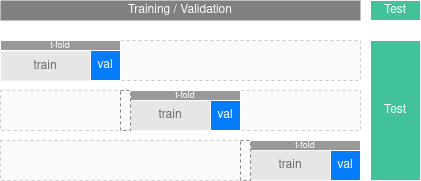
\includegraphics[width=18cm, height=10cm, keepaspectratio=true]{figures/T-Fold-SV.png}
      \end{figure}
        
    \end{block}
  \end{column}
  
  \begin{column}{.5 \textwidth - 0.01 \textwidth}
    \begin{block}{Information Representation and Sparsity Metric}
    
    \footnotesize
    A gamma distribution to fit the PDF of two set of variables, and the Kullback-Leibler Divergence to measure 
    the similarity between the two:
    \begin{equation}
      f(x) = \frac{\beta^{\alpha}}{\Gamma(\alpha)} x^{\alpha - 1}e^{-\beta x} \quad \text{for}
      \quad x > 0 \quad \alpha,\beta >0 
    \end{equation}
    
    $\Gamma(\alpha)$: The gamma function $\forall \ \alpha \in \mathbb{Z}^+$ and the
    $D_{KL}(P \vert\vert Q)$: Kullback-Liebler Divergence, which for unknown continuous random variables,
    $P, Q$, or for $p, q$ as empirically adjusted Probability Density Functions (PDF) is denoted by:
    \begin{equation}
        D_{KL}(P \vert\vert Q) = \int_{-\infty}^{\infty} p(x) log \Big( \frac{p(x)}{q(x)} \Big) dx 
    \end{equation}

    \end{block}
  \end{column}
  
\end{columns}

% -- -------------------------------------------------------------------------------------- ----------- -- %
% -- -------------------------------------------------------------------------------------- ----------- -- %

\begin{columns}[onlytextwidth]
  
  \begin{column}{.5 \textwidth - 0.01 \textwidth}
    \begin{block}{Predictive Modeling: Part 1}
        
      One common component of the predictive modeling process is binary-logloss cost function 
      with \textit{elasticnet} regularization:

      \begin{equation}
          J(w) =  J(w) + C \frac{\lambda}{m} \sum_{j=1}^n \left \lVert w_j \right\rVert_1 + (1 - C)
          \frac{\lambda}{2m} \sum_{j=1}^n \left \lVert w_j \right\rVert_2^2
      \end{equation}

      \footnotesize
      \noindent
      $L_{1}$: Also known as $Lasso$  \\
      $L_{2}$: Also known as $Ridge$ \\
      $C$: A coefficient to regulate the effect between $L_{1}$ and $L_{2}$
        
    \end{block}
  \end{column}

  \begin{column}{.5 \textwidth - 0.01 \textwidth}
    \begin{block}{Predictive Modeling: Part 2}
    
      Two models were defined, Logistic-Regression and Multi-layer Feedforward Perceptron. 
      
      \begin{table}[h]
      \small
      \begin{minipage}[h]{0.49\textwidth}
        \centering
        \begin{tabular}{@{}lll@{}}
            \hline
            \multicolumn{1}{c}{\textbf{Metric}} & \multicolumn{1}{c}{\textbf{ann-mlp}} &
            \multicolumn{1}{c}{\textbf{logistic}} \\ \hline
            acc-train & 0.9155 & 0.8311 \\ \hline
            acc-val & 0.8245 & 0.7368 \\ \hline
            acc-weighted & 0.4486 & 0.4061 \\ \hline
            acc-inv-weighted & 0.4213 & 0.3778 \\ \hline
            auc-train & 0.9924 & 0.9300 \\ \hline
            auc-val & 0.8401 & 0.8017 \\ \hline
        \end{tabular}
      \end{minipage}
      \begin{minipage}[h]{0.49\textwidth}
        \centering
        \begin{tabular}{@{}lll@{}}
            \hline
            \multicolumn{1}{c}{\textbf{Metric}} & \multicolumn{1}{c}{\textbf{ann-mlp}} &
            \multicolumn{1}{c}{\textbf{logistic}} \\ \hline
            auc-weighted & 0.4810 & 0.4521 \\ \hline
            auc-inv-weighted & 0.4353 & 0.4137 \\ \hline
            logloss-train & 0.2290 & 5.8333 \\ \hline
            logloss-val & 6.0595 & 9.0892 \\ \hline
            logloss-weighted & 0.6975 & 3.2422 \\ \hline
            logloss-inv-weighted & 2.4467 & 4.2190 \\ \hline
        \end{tabular}
      \end{minipage}
\end{table}
      
    \end{block}
  \end{column}
  
\end{columns}

% -- -------------------------------------------------------------------------------------- ----------- -- %
% -- -------------------------------------------------------------------------------------- ----------- -- %

\begin{columns}[onlytextwidth]
  
  \begin{column}{.25 \textwidth - 0.01 \textwidth}
    \begin{block}{Repository}
        
        For more information about the code implementation, data, and file templates go to the GitHub
        repository for this work.
        
        - github.com/IFFranciscoME/EcoSta2021
        
    \end{block}
  \end{column}
  
  \begin{column}{.75 \textwidth - 0.01 \textwidth}
    \begin{block}{References}
    
    \begin{thebibliography}{02}
      \bibitem{Lopez-de-Prado-AFML-2018}
              Lopez de Prado, Marcos M (2018), \textit{Advances in Financial Machine Learning}, \emph{Wiley}.

      \bibitem{Pezeshki-GS-2020}
               Pezeshki et al (2020). \textit{Gradient Starvation:A Learning Proclivity in Neural Networks},
               Mohammad Pezeshki, Sekou-Oumar Kaba, Yoshua Bengio, Aaron Courville, Doina Precup,
               Guillaume Lajoie, arXiv:2011.09468.
                                                     
      \bibitem{Goodfellow-et-al-DL-2017}
               Goddfellow et al (2017), \textit{Deep Learning}, Ian Goodfellow, Yoshua Bengio,
               Aaron Courville, MIT Press
    \end{thebibliography}
    
    \end{block}
  \end{column}
\end{columns}

% -- -------------------------------------------------------------------------------------- ----------- -- %
% -- -------------------------------------------------------------------------------------- ----------- -- %

\begin{columns}[onlytextwidth]
  
  \begin{column}{1 \textwidth - 0.01 \textwidth}
    \begin{block}{Additional Row-Block}
        
      Additional content inside block
        
    \end{block}
  \end{column}
\end{columns}

\end{frame}
\end{document}
